\section{Optimized Implementation}
\label{sec4}
Calculating LA in the specific format detailed in Section~\ref{sec3} offers the potential to increase both the data reuse rate (the number of times each element is used per off-chip memory access) and parallelization. Specifically, the operations are ordered to ensure that each data segment is accessed by a single thread. This ordering prevents scenarios where multiple threads conflict over the same element or where individual threads require data exceeding the shared memory (L1 cache) size, thereby preventing redundant off-chip memory accesses. In this section we will provide the details of our optimized CUDA implementation such as data movement and thread scheduling for the forward and backward-pass. We employ attention kernel of $f(x) = 1 + x$, and the variables are stored as three dimensional tensors.

\subsection{Forward-Pass}
To calculate the output $\mathbf{O}$, we require $\mathbf{f}_{ij}$ and $\mathbf{g}_i$, where $\mathbf{f}_{ij}$ and $\mathbf{g}_i$ are obtained according to Equation~\ref{fglast}. We will detail the process for calculating $\mathbf{f}_{ij}$, and $\mathbf{g}_i$ follows a similar, simpler process. 
\par To derive $\mathbf{f}_{ij}$, we need to find two sets of coefficients $x^{(1)}$ and $x^{(2)}$, as described by Equation~\ref{xy}. The derivation of $x^{(1)}$ and $x^{(2)}$ is sequential, meaning that $x^{(1)}_{ij}$ and $x^{(2)}_{ijm}$ depend on $x^{(1)}_{i-1j}$ and $x^{(2)}_{i-1j}$. As a result, the derivation of each individual $x^{(1)}_{ij}$ and $x^{(2)}_{ijm}$ cannot be parallelized; at least not without employing `\textit{reduction}`  techniques\footnote{\url{https://developer.download.nvidia.com/assets/cuda/files/reduction.pdf}}. For now, let's assume a non-parallelized approach. Similarly, the derivation of each individual $f_{ij}$ is also inherently sequential. Therefore, the computation of $x^{(1)}_{ij}$, $x^{(2)}_{ijm}$ and $f_{ij}$ for each $j$ should be performed within the same thread as well.

\par As a reminder $\mathbf{f}_{ij}$ is calculated as 
\begin{gather}
    \mathbf{f}_{ij} = x^{(1)}_j + \sum_{m=1}^{D}{\mathbf{q}_{im}x^{(2)}_{jm}},
\end{gather}
which we refer to the left term $x^{(1)}_j$ as the Constant term and the right term $\sum_{m=1}^{D}{\mathbf{q}_{i,m}x^{(2)}_{jm}}$ as the Linear term. Let's first proceed with the Constant term. We call $D$ threads for $1\leq j\leq D$, in each thread perform a loop for $1\leq i\leq N$ to calculate $x^{(1)}_{ij}$, and assign it to $f_{ij}$ as shown in Algorithm~\ref{alg1} in the Appendix. Since the $x^{(1)}_{ij}$ values for each $j$ is only accessed within a thread, we can use a single register to store and update the $x^{(1)}_{ij}$ values in the for loop, rather than store them for each $i$. This will accelerate the read operations (accessing in-thread registers is considerably faster than accessing shared memory) and reduce the memory consumption. Furthermore, each thread $j$ will access the off-chip memory to read the $\mathbf{v}_{ij}$ values for $1\leq i\leq N$, and to write $\mathbf{f}_{ij}$. To leverage the efficient data movement capabilities of NVIDIA GPU Streaming Multiprocessors (SMs), which fetch adjacent data blocks from off-chip memory to the L2 and L1 caches for adjacent blocks and threads, the $\mathbf{V}_{ij}$ and $\mathbf{f}_{ij}$ values should be stored with $j$ as the first tensor dimension and $i$ as the second.

% \begin{algorithm}
% \caption{Forward-Pass, Constant Term (left) and Linear Term (right)}
% \begin{minipage}{0.49\textwidth}
% \begin{spacing}{1}
%   \label{alg1}
%   \begin{algorithmic}[1] % The [1] adds line numbers
%   \STATE \textbf{Input:} v $\in \mathbb{R}^{B\times H,\,N,\,D}$
%   \STATE \textbf{Output:} f $\in \mathbb{R}^{B\times H,\,N,\,D}$
%     \STATE \textbf{Call} $B\times H$ blocks ($1\leq bh\leq B\times H$)
%     \STATE \textbf{Call} $D$ threads in each block ($1\leq j\leq D$) 
%     \STATE In each thread:
%     \STATE x = 0 (on-thread register)
%     \FOR {$i \gets 1$ \TO $N$}
%        \STATE x += v[$bh$][$i$][$j$]
%        \STATE f[$bh$][$i$][$j$] = x
%     \ENDFOR
%   \end{algorithmic}
%   \end{spacing}
% \end{minipage}
% % \end{algorithm}
% \hfill % Pushes the two minipages apart
% % \begin{algorithm}[!h]
% \begin{minipage}{0.49\textwidth}
% \begin{spacing}{1}
%   \label{alg2}
%   \begin{algorithmic}[1] % The [1] adds line numbers
%     \STATE \textbf{Input:} q, k, v $\in \mathbb{R}^{B\times H,\,N,\,D}$
%     \STATE \textbf{Output:} f $\in \mathbb{R}^{B\times H,\,N,\,D}$
%     \STATE \textbf{Call} $B\times H$ outer blocks ($1\leq bh\leq B\times H$)
%     \STATE \textbf{Call} $L$ inner blocks ($1\leq l\leq L$)
%     \STATE \textbf{Call} $D$ threads in each block ($1\leq j\leq D$) 
%     \STATE In each thread:
%     \STATE vr, x = 0 (on-thread register)
%     \STATE r[$1$ to $D/L$] = 0 (on-thread register)
%     \STATE sq[$1$ to $D$] = 0 (shared memory)
%     \STATE sk[$1$ to $D$] = 0 (shared memory)
%     \FOR {$i \gets 1$ \TO $N$}
%         \STATE x = 0
%         \STATE vr = v[$bh$][$i$][$j$]
%         \STATE \textbf{load} k[$bh$][$i$][$j$] \textbf{to} sk[$j$]
%         \STATE \textbf{load} q[$bh$][$i$][$j$] \textbf{to} sq[$j$]
%        \FOR {$m \gets 1$ \TO $D/L$}
%            \STATE r[$m$] += vr$\times$sk[$l\times D/L + m$]
%            \STATE x += r[$m$]$\times$sq[$l\times D/L + m$]
%        \ENDFOR
%        \STATE f[bh][i][j] += x
%     \ENDFOR
%   \end{algorithmic}
%   \end{spacing}
%   \end{minipage}
% \end{algorithm}



\par To calculate the Linear term, we call $D$ threads for $1\leq j\leq D$, and in each thread perform a loop for $1\leq m\leq D$ within a loop for $1\leq i\leq N$ to calculate $x^{(2)}_{ijm}$ and add it to $f_{ij}$, as shown in Algorithm~\ref{alg2}. Since the $x^{(2)}_{ijm}$ values for each $j$ are only accessed within a thread, we can use an array of registers to store them for each $m$, and sequentially update it as the $x^{(2)}_{ijm}$ values to accelerate read operations. However, the value of $D$ is often too large for the whole $x^{(2)}_{ijm}$ $1\leq m\leq D$ to be stored in thread registers. As a workaround we perform reduction, where we break the inner loop into separate $L$ block of threads, that is, we call $L$ blocks, each with $D$ threads, and in each thread performing loop for $1\leq m\leq D/L$ within a loop for $1\leq i\leq N$. By applying reduction, multiple threads might edit the same $f_{ij}$, and therefore we would have to use `Race Aware` operations when updating $f_{ij}$. We use $L=\dfrac{D}{32}$ in our implementation.

\par Furthermore, since the $\mathbf{q}_{im}$ and $\mathbf{k}_{im}$ values for each $m$ are accessed within the same block of threads, we can store them in shared memory (note that multiple block of threads will access the same $\mathbf{q}_{im}$ and $\mathbf{k}_{im}$). To be specific, within every iteration of the outer loop (for $1\leq i\leq n$), each thread moves one element of $\mathbf{q}$ and $\mathbf{k}$ from the off-chip memory to the shared memory; a total of $2\times D$ elements. Since $64\leq D\leq 512$, there is enough shared memory for storage. In order to enable the adjacent threads utilize the shared memory, corresponding $\mathbf{q}_{im}$ and $\mathbf{k}_{im}$ values should be stored with $m$ as the first tensor dimension and $i$ as the second. By parallelizing the read operations and utilizing shared memory, we reduce the read time from $ND\,t_{oc}$ to $N,t_{oc} + D\,t_{s}$, where $t_{oc}$ and $t_{s}$ are the read time for off-chip and shared memory ( $t_{s}<< t_{oc}$). For context, $t_{oc}$ is on the order of a hundred cycles, where $t_{s}$ a few cycles.


\par Finally, considering the multiple attention heads $H$ in each Transformer layer and multiple input batches $B$, the entire process is executed across $B\times H$ parallel blocks. The values are stored such that the third tensor dimension corresponds to the batch and head numbers. Overall, the process involves $B\times H$ outer blocks, $L$ inner blocks, and $D$ threads per block. For instance, Figure~\ref{figmemory} illustrates the structure of the $\mathbf{q}_{rij}$ values and the data movement pattern for calculating the Linear term with a batch size of $B=2$, number of heads $H=4$, dimension per head $D=6$, sequence length $N=8$, and \textit{reduction} block size $L=2$ (indicated as A and B blocks), where $1\leq r\leq B\times H$, $1\leq i\leq N$, and $1\leq j\leq D$. Cells sharing the same color belong to the same outer block, cells with the same letter (A or B) belong to the same inner block, and each cell within an inner block is accessed by D threads. The $\mathbf{q}$ cells are then processed sequentially, with the left number in each cell indicating the outer loop iteration (line 11 in Algorithm~\ref{alg2}) and the right number indicating the inner loop iteration (line 16 in Algorithm~\ref{alg2}). In a 1-dimensional view, the data are arranged so that data processed by adjacent threads are spatially adjacent. For example, cells with the same color and the same letter are positioned next to each other.
\par Note that the data movement differs for other tensors such as $\mathbf{k}$ and $\mathbf{v}$. We should also mention that we must ensure threads related to the Constant term complete their execution before invoking threads related to the Linear term to prevent race conditions, as both sets of threads might modify the same $f_{ij}$. 


\begin{figure}[h]
\begin{centering}
  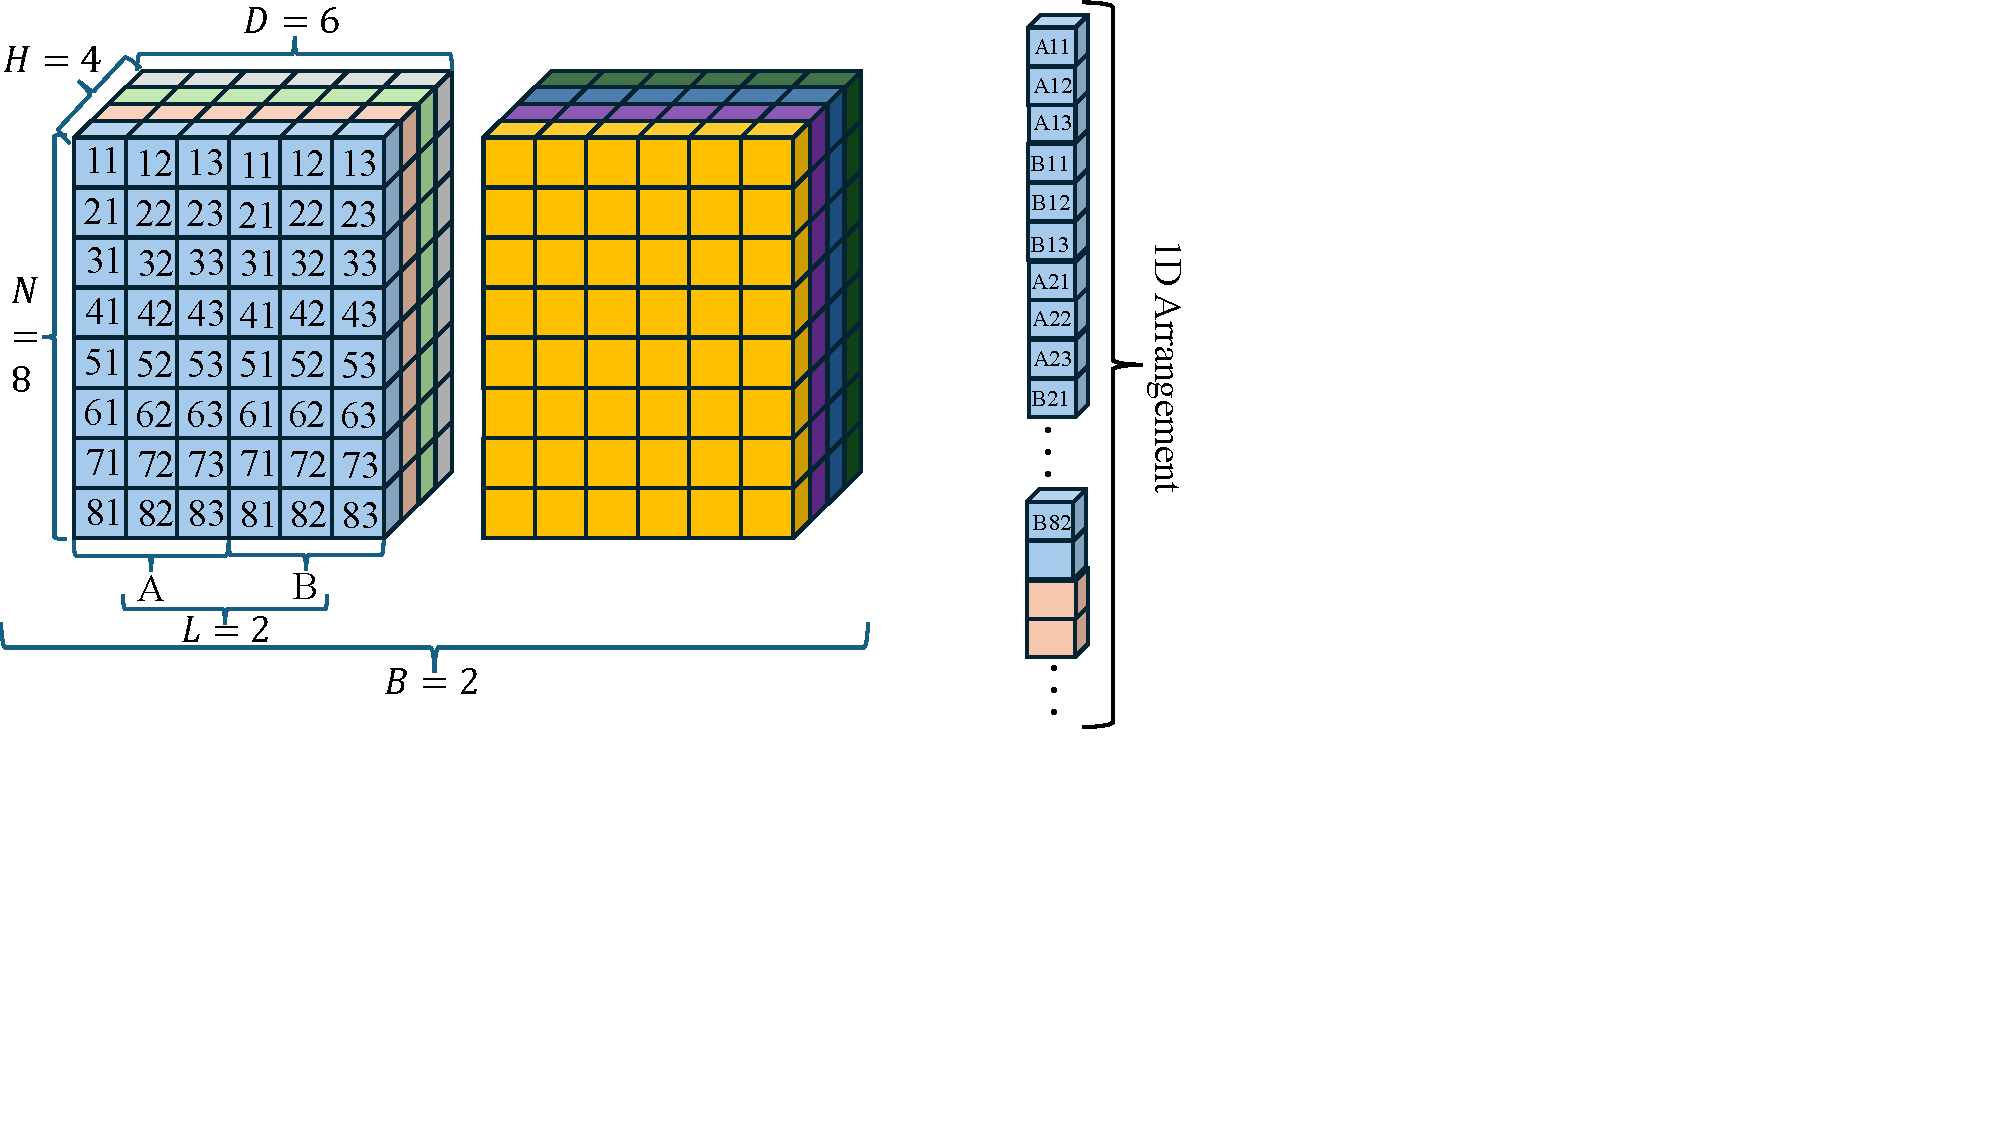
\includegraphics[width=0.8\linewidth, trim=0mm 60mm 135mm 0mm, clip=true]{images/memory.pdf}
\vspace{-15pt}
\caption{Structure of the Query ($\mathbf{Q}$) storage and its data movement pattern for calculating the Linear term with a batch size of $B=2$, number of heads $H=4$, dimension per head $D=6$, sequence length $N=8$, and \textit{reduction} block size $L=2$. Cells with the same color and letter (A or B) are processed by the same block of threads, and the left and right numbers on each cell denote the sequential order of processing in each thread's outer and inner loops.}
\label{figmemory}
\end{centering}
\end{figure}

\subsection{Backward-Pass}
During the backward-pass, the attention layer takes the incoming gradient of the layer in front, and produces the gradient with respect to $\mathbf{Q}$, $\mathbf{K}$ and $\mathbf{V}$, as shown in Equations~\ref{back1}-\ref{back2}. We will detail the process for calculating the gradient with respect to $\mathbf{K}$ ($\nabla_{\mathbf{K}}\mathbf{\Psi}$), and $\nabla_{\mathbf{Q}}\mathbf{\Psi},\,\nabla_{\mathbf{V}}\mathbf{\Psi}$ follows a similar process. To derive $\mathbf{f}_{ij}$, we need to find two sets of coefficients $\alpha^{K}$ and $\beta^{K}$. Similar to the forward-pass, these coefficients are determined sequentially, as described by Equation~\ref{endd}. As a reminder $\nabla_{\mathbf{k}_{ir}}\mathbf{\Psi}$ is calculated as
\begin{gather}
    \nabla_{\mathbf{k}_{ij}}\mathbf{\Psi} = \sum_{m=1}^{D}\alpha_{ijm}^{K}\,\mathbf{v}_{im} - \sum_{m=1}^{D}\beta_{ijm}^{K},
\end{gather}
where we refer to the left term $\sum_{m=1}^{D}\alpha_{ijm}^{K}\,\mathbf{v}_{im}$ as the Alpha term, and the right term $\sum_{m=1}^{D}\beta_{ijm}^{K}$ the Beta term. To derive them, we take an approach similar to calculation of Linear term in forward-pass; to call $B\times H$ outer blocks, $L$ inner blocks, and $D$ threads per block.

\par To calculate the Alpha term, each thread consists of an outer loop for $1\leq i\leq N$ and an inner loop for $1\leq m\leq D/L$. The $\alpha_{ijm}^{K}$ are then calculated sequentially and assigned to $\nabla_{\mathbf{k}_{ij}}\mathbf{\Psi}$, as shown in Algorithm~\ref{alg3}. Given that the $\mathbf{q}_{ij}$ values for each $j$ are solely accessed within a thread, we can use a single register to store and update them in the for loop. Furthermore, since the $\alpha_{ijm}^{K}$ values are accessed only within a thread as well, we use an array of registers to store them, employing the same \textit{reduction} techniques to manage the limited register space.

\par The $\mathbf{v}_{im}$ and $\mathbf{\hat{\Omega}}_{im}$ for each $m$ are accessed within the same block of threads. Therefore, we can store them in shared memory. Analogous to the Linear terms in forward pass, the data movement from the off-chip to shared memory is parallelized among each block of threads to reduce the read time from $ND\,t_{oc}$ to $N,t_{oc} + D\,t_{s}$. To optimize data movement for $\mathbf{\hat{\Omega}}_{ij}$ and $\nabla_{\mathbf{k}_{ij}}\mathbf{\Psi}$ by the SMs, we should store them with $m$ and $i$ mapping to the first and second tensor dimensions respectively. This arrangement allows adjacent threads to access adjacent memory, enhancing efficiency.


% \begin{algorithm}
% \caption{Backward-Pass, Alpha Term (left) and Beta Term (right)}
% \begin{minipage}{0.49\textwidth}
% \begin{spacing}{1}
%   \label{alg3}
%   \begin{algorithmic}[1] % The [1] adds line numbers
%     \STATE \textbf{Input:} q, v, $\hat{\Omega}$ $\in \mathbb{R}^{B\times H,\,N,\,D}$
%     \STATE \textbf{Output:} $\nabla_{\mathbf{k}}\mathbf{\Psi}$ $\in \mathbb{R}^{B\times H,\,N,\,D}$
%     \STATE \textbf{Call} $B\times H$ outer blocks ($1\leq bh\leq B\times H$)
%     \STATE \textbf{Call} $L$ inner blocks ($1\leq l\leq L$)
%     \STATE \textbf{Call} $D$ threads in each block ($1\leq j\leq D$) 
%     \STATE In each thread:
%     \STATE qr, x = 0 (on-thread register)
%     \STATE r[$1$ to $D/L$] = 0 (on-thread register)
%     \STATE sv[$1$ to $D$] = 0 (shared memory)
%     \STATE sg[$1$ to $D$] = 0 (shared memory)
%     \FOR {$i \gets N$ \TO $1$}
%         \STATE x = 0
%         \STATE qr = q[$bh$][$i$][$j$]
%         \STATE \textbf{load} v[$bh$][$i$][$j$] \textbf{to} sv[$j$]
%         \STATE \textbf{load} $\hat{\Omega}$[$bh$][$i$][$j$] \textbf{to} sg[$j$]
%        \FOR {$m \gets 1$ \TO $D/L$}
%            \STATE r[$m$] += qr$\times$sg[$l\times D/L + m$]
%            \STATE x += r[$m$]$\times$sv[$l\times D/L + m$]
%        \ENDFOR
%        \STATE $\nabla_{\mathbf{k}}\mathbf{\Psi}$[bh][i][j] = x
%     \ENDFOR
%   \end{algorithmic}
%   \end{spacing}
% \end{minipage}
% % \end{algorithm}
% \hfill % Pushes the two minipages apart
% % \begin{algorithm}[!h]
% \begin{minipage}{0.49\textwidth}
% \begin{spacing}{1}
%   % \caption{Backward-Pass, Beta term}
%   \label{alg4}
%   \begin{algorithmic}[1] % The [1] adds line numbers
%     \STATE \textbf{Input:} q, v, $\hat{\Omega}$ $\in \mathbb{R}^{B\times H,\,N,\,D}$
%     \STATE \textbf{Output:} $\nabla_{\mathbf{k}}\mathbf{\Psi}$ $\in \mathbb{R}^{B\times H,\,N,\,D}$
%     \STATE \textbf{Call} $B\times H$ outer blocks ($1\leq bh\leq B\times H$)
%     \STATE \textbf{Call} $L$ inner blocks ($1\leq l\leq L$)
%     \STATE \textbf{Call} $D$ threads in each block ($1\leq j\leq D$) 
%     \STATE In each thread:
%     \STATE qr, x = 0 (on-thread register)
%     \STATE r[$1$ to $D/L$] = 0 (on-thread register)
%     \STATE so[$1$ to $D$] = 0 (shared memory)
%     \STATE sg[$1$ to $D$] = 0 (shared memory)
%     \FOR {$i \gets N$ \TO $1$}
%         \STATE x = 0
%         \STATE qr = q[$bh$][$i$][$j$]
%         \STATE \textbf{load} o[$bh$][$i$][$j$] \textbf{to} so[$j$]
%         \STATE \textbf{load} $\hat{\Omega}$[$bh$][$i$][$j$] \textbf{to} sg[$j$]
%        \FOR {$m \gets 1$ \TO $D/L$}
%            \STATE r[$m$] += qr$\times$sg[$l\times D/L + m$]$\times$so[$l\times D/L + m$]
%            \STATE x += r[$m$]
%        \ENDFOR
%        \STATE $\nabla_{\mathbf{k}}\mathbf{\Psi}$[bh][i][j] -= x
%     \ENDFOR
%   \end{algorithmic}
%   \end{spacing}
%   \end{minipage}
% \end{algorithm}


\par Similarly, to calculate the Beta term, each thread consists of an outer loop for $1\leq i\leq N$ and an inner loop for $1\leq m\leq D/L$, where the $\beta{ijm}^{K}$ are calculated sequentially and deducted from $\nabla_{\mathbf{k}_{ij}}\mathbf{\Psi}$, as shown in Algorithm~\ref{alg4}. The main difference compared to Alpha term calculation is that instead of storing $\mathbf{v}_{im}$ and $\mathbf{\hat{\Omega}}_{im}$ in the shared memory, $\mathbf{o}_{im}$ and $\mathbf{\hat{\Omega}}_{im}$ will be stored.




